% !TeX spellcheck = de_DE
\chapter{The Proposed Solution}
This chapter gives a detailed explanation of the proposed approach and the various steps involved in it. It elaborates on the theoretical design behind the conversion of agile requirements described in natural language into formal models and the subsequent test case generation methodologies.
 
The first section of this chapter gives an overview of the proposed solution and the different steps involved in it. The following sections elaborate the steps defined in the overview and the justification on which the theoretical ideas are chosen.


\section{Overview of the solution}
The proposed solution of test script generation from requirements can be broadly classified into four important steps.
\begin{enumerate}
\item Requirements in a Restricted Natural Language.
\item Generation of Petri-Nets from Use Case Specifications.
\item Generation of Reachability/Coverability Graph.
\item Generation of Test Specifications and Test Scripts.
\end{enumerate}
Figure \ref{fig:proposed_solution2} shows the skeleton of the proposed work. The detailed explanation of these steps can be found in the following sections.

\begin{figure}[]
\centering
\fbox{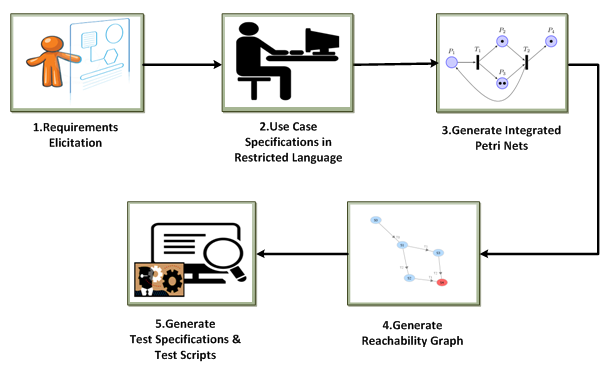
\includegraphics[width=0.9\textwidth]{content/images/Chapter4/proposed_solution.png}}
\caption{An overview of the proposed solution}
\label{fig:proposed_solution2}
\end{figure}


\section{Requirements in a Restricted Natural Language}
The main objective of this approach is to generate test cases directly from requirements specified in natural language. In the industry, one of the important documents used to communicate requirements between the different stakeholders is \glspl{ucs}. In order to reduce the incompleteness and imprecision in \glspl{ucs}, a template with restriction rules are usually used, thereby making it a semi-formal representation. 

\subsection{RUCM – A Restricted Natural Language}
\gls{rucm} \cite{yue2013facilitating} is one such use case format that provides restriction rules and specific keywords, hence confining the use of natural language for \glspl{ucs}. It also corresponds to a specific metamodel called UCMeta, which facilitates automatic analysis of use cases. The selection of a restricted \gls{nl} template depends upon factors like simplicity, expressive power, better understandability and quality of models derived from it. Experiment results \cite{yue2013facilitating} shows that the template is beneficial and is applicable in various scenarios with the above mentioned characteristics.

\subsection{Restriction Rules and Keywords}
\gls{rucm} has also defined a list of standard keywords. A short overview of the rules is given below. For example, a conditional logic sentence is defined by the keyword IF-THEN-ELSEIF-ELSE-ENDIF, a concurrency statement by keyword MEANWHILE, condition checking sentences by keyword VALIDATES THAT and iteration sentences by DO-UNTIL. RESUME STEP keyword is used when the alternative flow should return back to its reference flow. Similarly, ABORT keyword is used to describe an exit action due to some exceptions.  The complete set of keywords can be found in the template reference given in \cite{yue2013facilitating}. In addition to the keywords, \gls{rucm} also specifies restriction rules that are detailed in \cite{yue2013facilitating}. A table describing the basic elements of a \gls{rucm} template is given in Table \ref{tab:rucmtemplate}.

% Table generated by Excel2LaTeX from sheet 'Sheet1'
\begin{table}[htbp]
  \centering
  \caption{RUCM Use Case Template}
	\begin{adjustbox}{width=1\textwidth}
    \begin{tabular}{|l|l|l|l|l|l|l|l|}
    \toprule
    Element & \multicolumn{7}{l|}{ Description} \\
    \midrule
    Use Case Name & \multicolumn{7}{l|}{ The name of the use case. It usually starts with a verb.} \\
    \midrule
    Brief Description  & \multicolumn{7}{l|}{Summarizes the use case in a short paragraph.} \\
    \midrule
    Precondition & \multicolumn{7}{l|}{ What should be true before the use case is executed.} \\
    \midrule
    Primary Actor  & \multicolumn{7}{l|}{The actor which initiates the use case.} \\
    \midrule
    Secondary Actors & \multicolumn{7}{l|}{ Other actors the system relies on to accomplish the services of the use case.} \\
    \midrule
    Dependency & \multicolumn{7}{l|}{ Include and extend relationships to other use cases.} \\
    \midrule
    Generalization & \multicolumn{7}{l|}{ Generalization relationships to other use cases.} \\
    \midrule
    \multirow{3}[6]{*}{Basic Flow} & \multicolumn{7}{l|}{ Specifies the main successful path, also called “happy path.”} \\
\cmidrule{2-8}          & \textbf{Steps (numbered) } & \multicolumn{6}{l|}{Flow of events.} \\
\cmidrule{2-8}          & \textbf{Postcondition} & \multicolumn{6}{l|}{ What should be true after the basic flow executes.} \\
    \midrule
    \multicolumn{1}{|l|}{\multirow{4}[8]{*}{Specific \newline{}Alternative Flows}} & \multicolumn{7}{l|}{Applies to one specific step of the basic flow.} \\
\cmidrule{2-8}          & \textbf{RFS} & \multicolumn{6}{l|}{ A reference flow step number where flow branches from.} \\
\cmidrule{2-8}          & \textbf{Steps (numbered)} & \multicolumn{6}{l|}{ Flow of events.} \\
\cmidrule{2-8}          & \textbf{Postcondition} & \multicolumn{6}{l|}{ What should be true after the alternative flow executes.} \\
    \midrule
    \multicolumn{1}{|l|}{\multirow{3}[6]{*}{Global Alternative\newline{} Flows}} & \multicolumn{7}{l|}{ Applies to all the steps of the basic flow.} \\
\cmidrule{2-8}          & \textbf{Steps (numbered)} & \multicolumn{6}{l|}{ Flow of events.} \\
\cmidrule{2-8}          & \textbf{Postcondition} & \multicolumn{6}{l|}{ What should be true after the alternative flow executes.} \\
    \midrule
    \multicolumn{1}{|l|}{\multirow{4}[8]{*}{Bounded \newline{}Alternative Flows}} & \multicolumn{7}{l|}{Applies to more than one step of the basic flow, but not all of them.} \\
\cmidrule{2-8}          & \textbf{RFS} & \multicolumn{6}{l|}{ A list of reference flow steps where flow branches from.} \\
\cmidrule{2-8}          & \textbf{Steps (numbered)} & \multicolumn{6}{l|}{ Flow of events.} \\
\cmidrule{2-8}          & \textbf{Postcondition} & \multicolumn{6}{l|}{ What should be true after the alternative flow executes.} \\
    \bottomrule
    \end{tabular}%
	\end{adjustbox}
  \label{tab:rucmtemplate}%
\end{table}%


\gls{rucm} was basically created for analysis of use cases and not for test case generation. Hence few additional restrictions were added to \gls{rucm} by the authors of \cite{wang2015umtg}. In order to establish composite conditions with multiple specific alternative flows, the authors decided that the specific alternative flow should also begin with the keyword IF....THEN.  Further additions to the restriction rules can be found in \cite{wang2015umtg}. This work has also made some assumptions and changes to the \gls{rucm} template which will be detailed in Chapter \ref{implementation}.
 
\subsection{Comparison with a related RNL}
Another widely used Restricted Natural Language Specification is the Scenario Specifications. It also uses restricted vocabulary and introduces restriction rules similar to \gls{rucm}. According to the author in \cite{calisaya2016analysis}, a scenario is a collection of partially ordered event occurrences, each guarded by a set of conditions (pre or post) or restricted by constraints. Further details on the scenario specifications can be found in the literature (\cite{do2000scenario}, \cite{calisaya2016analysis}).

An initial comparison between the two templates revealed the following conclusions. Scenario Specification is deprived of certain properties like the metamodel defined is not exhaustive and hence it cannot be used for complete test case generation. \gls{rucm} is more suited for safety critical embedded software and an industrial case study with this template yielded good results \cite{wang2015umtg}. Test data generation is easier with the help of \gls{rucm} since natural language processing can be introduced early in the process because of the detailed metamodel. 

Scenario Specification, on the other hand, has been used to specify requirements in natural language and subsequently to automate the check of correctness, consistency, completeness and unambiguity properties of the requirements in \cite{calisaya2016analysis}. The work in the mentioned literature also makes use of Petri Nets as a formal model for the analysis. This work uses \gls{rucm} as a template for \gls{rnl} requirement specifications and the work using Scenario Specifications as a foundation for transformation to formal models. 


\section{Generation of Petri Nets from Use Case Specifications}\label{integratedpngen}
One of the main objectives of this work is to establish a formal model for the requirements specified in natural language. The formal model in our work is Petri Nets, to be precise Place-Transition Petri Net, which is a sub category of Petri Nets. To establish the conversion from \gls{ucs} to PN, we use the concept of Model-to-Model (M2M) transformations. For this purpose, the \glspl{ucs} are described as a metamodel and we use \gls{rucm} as a template for this. Petri Net, on the other hand, can also be described as a metamodel.

The transformation method from \gls{ucs} to PN consists of three main steps.

\begin{enumerate}
\item The first step defines mapping rules that translate the \gls{rucm} elements into corresponding Petri Net elements according to transformation rules defined in Figure \ref{fig:rules}. The expected result of this process is a Sub Petri Net which consists of at least one place, transition and arc.
\item The second step is to compose the sub Petri Nets generated from the previous step into a whole Petri Net. This is done by the fusion of output and input dummy places between sequential sub Petri Nets or by integrating Petri Nets of other referenced \glspl{ucs}.
\item The third step is to generate an integrated Petri Net from the partial Petri Nets generated for each \gls{ucs}. According to \gls{rucm} specification, each \gls{ucs} can reference another \gls{ucs} and hence the need arises to transform referenced \gls{ucs} into a Petri Net. This step integrates the partial Petri Nets into an Integrated Petri Net and hence it reflects the properties of the synthesized partial Petri Nets.
\end{enumerate}

%\begin{figure}[htb!]
%\centering
%\fbox{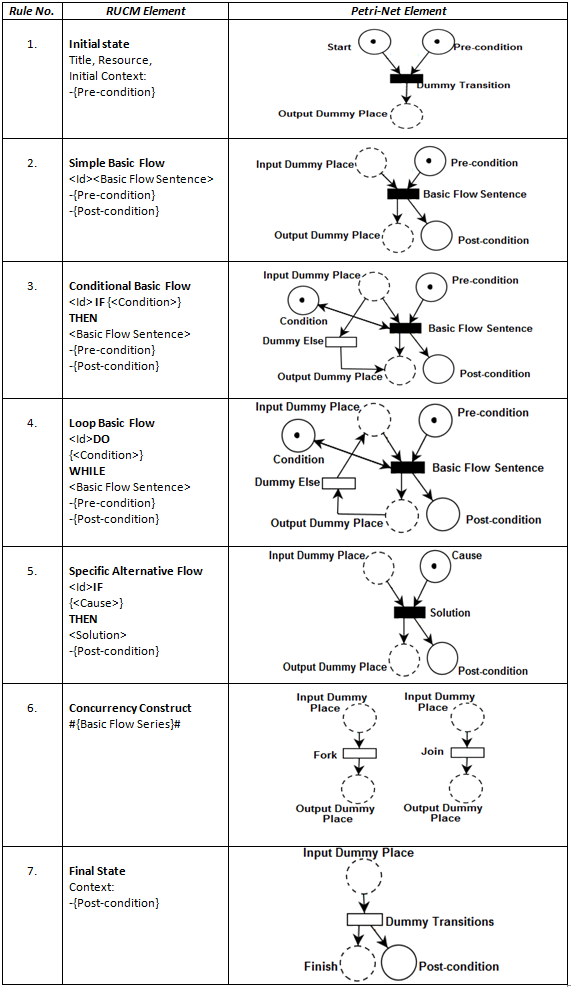
\includegraphics[width=0.8\textwidth]{content/images/Chapter4/Rules.png}}
%\caption{Model-to-Model(M2M) Transformation Rules}
%\label{fig:rules}
%\end{figure}


The different transformations and metamodels are detailed in Chapter \ref{implementation} along with a running example. As a result of the above transformations, we obtain a Petri Net that is equivalent for the given \gls{ucs}.

\begin{figure}[htb!]
  \centering
    \subfloat[first transition]{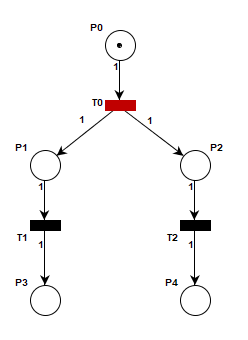
\includegraphics[width=0.3\textwidth,frame]{content/images/Chapter4/first.png} \label{fig:rg_subfigA}}
   \subfloat[second transition]{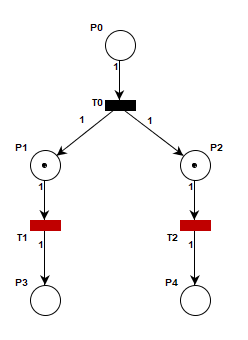
\includegraphics[width=0.3\textwidth,frame]{content/images/Chapter4/second.png} \label{fig:rg_subfigB}}
   
     \subfloat[third transition]{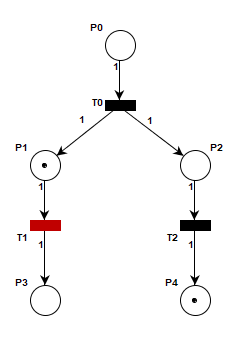
\includegraphics[width=0.3\textwidth,frame]{content/images/Chapter4/third.png} \label{fig:rg_subfigC}}
   \subfloat[fourth transition]{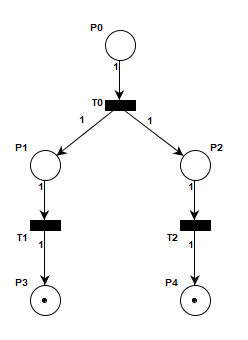
\includegraphics[width=0.3\textwidth,frame]{content/images/Chapter4/fourth.png} \label{fig:rg_subfigD}}
	\caption{Concept of Reachability.}
\label{fig:rgconcept}
\end{figure}

\section{Generation of Reachability/Coverability Graph}
As mentioned in Chapter \ref{background}, one of the important properties of Petri Net for dynamic analysis is reachability. As already described, when a transition is enabled for firing, tokens are transferred between places. This causes a change in marking of the Petri Net and each marking is defined by the term \textit{state}. Thus a new state is reached from the initial state. A \textit{reachable state} is defined as a state that can be reached from the current state (marking).

The Figure \ref{fig:rgconcept} explains the above process with the help of Petri Nets. The firing sequence of transitions described in the figure is $ \lbrace $T0, T2, T1$ \rbrace $. Initial marking of the Petri Net is given by $ \lbrace $1, 0, 0, 0, 0$ \rbrace $ which corresponds to $ \lbrace $P0, P1, P2, P3, P4$ \rbrace $. After the first firing, the marking of the Petri Net changes to $ \lbrace $0, 1, 1, 0, 0$ \rbrace $. As defined, these markings are also termed as states and in our case, they are termed as S0 and S1 respectively. Hence it can be seen that S1 is a reachable state from S0.

A reachability or coverability graph is a graph that contains reachable markings or states as nodes and transitions, which cause the flow of tokens, as arcs. This graph contains all the possible reachable states from the initial state and can even have multiple paths. Reachability graph for the configuration given in Figure \ref{fig:rg_subfigA} is shown in Figure \ref{fig:rgexp}. Here, it can be seen that for the state S1 there are two possible reachable states namely S2 and S3 and hence contains two paths. The path described in Figure \ref{fig:rg_subfigC} is $ \lbrace $S0, S1, S2, S4$ \rbrace $ whereas there is an additional path $ \lbrace $S0, S1, S3, S4$ \rbrace $ in the reachability graph.

\begin{figure}[htb!]
\centering
\fbox{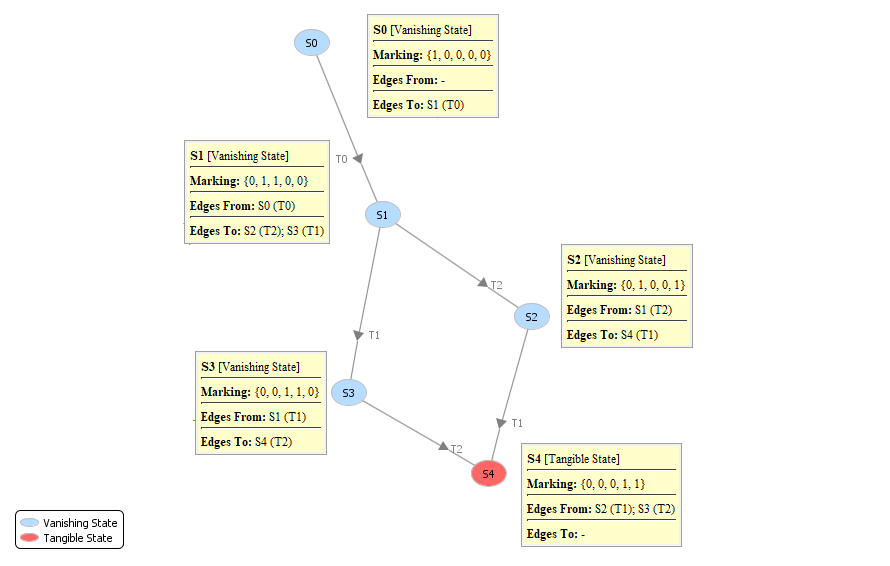
\includegraphics[scale=0.9]{content/images/Chapter4/fifth.png}}
\caption{An example of Reachability Graph}
\label{fig:rgexp}
\end{figure}

\section{Generation of Test Specifications and Test Scripts}
The Reachability Graph acts as an input for the generation of Test Specifications and Scripts. A Reachability Graph is composed of tangible and vanishing states with transitions (from Petri Nets) acting as arcs. A tangible state is a final reachable state from a given initial state whereas a vanishing state is a state that is traversed before reaching a tangible state. Now each path from the initial state to a tangible state forms a test scenario since each arc represents a transition from Petri Net. A test scenario is a sequence of actions performed to reach a particular state. In order to make these test scenarios into complete test specifications, we add other elements like Pre-Conditions, Post-Conditions and conditions from logical statements, etc. 

The test specifications consist of a set of test cases and each test case, in turn, is made up of a set of test steps. In practice, the test scripts are realized as a set of test steps that are implemented as packages in platform specific languages. A mapping table is created to map each of the test steps to specific packages in platform specific languages. For test data, the numerical values from test steps are extracted and used for test script generation.





